% Metódy inžinierskej práce

\documentclass{article}

%\usepackage[T1]{fontenc}
\usepackage[IL2]{fontenc} % lepšia sadzba písmena Ľ než v T1
\usepackage[utf8]{inputenc}
\usepackage{graphicx}
\usepackage{url} % príkaz \url na formátovanie URL
\usepackage{hyperref} % odkazy v texte budú aktívne (pri niektorých triedach dokumentov spôsobuje posun textu)
\usepackage{enumitem}  % For adjusting list spacing
\usepackage{indentfirst}
\usepackage{amsmath}
\usepackage{float}
\usepackage{tabularx}
\usepackage{array}
\usepackage{booktabs}
\usepackage{multirow}
\usepackage{multicol}
\usepackage{xcolor}

\usepackage{cite}
%\usepackage{times}
\usepackage{caption}
\captionsetup{labelsep=period}

\pagestyle{headings}

\title{Content-based filtering\thanks{Semester project in the subject Methods of engineering work. Year 2024/25, supervision: Pavol Baťalík}}

\author{Sladkovskyi Heorhii\\[2pt]
	{\small Slovak University of Technology in Bratislava}\\
	{\small Faculty of Informatics and Information Technologies STU in Bratislava}\\
	{\small \texttt{xsladkovskyi@stuba.sk}}
	}

\date{\small 14. december 2024}

\begin{document}

\maketitle

\begin{abstract}
    \ldots
\end{abstract}
\section{Introduction}\label{sec:introduction}

\subsection{Definition}% Definition of Content-Based Filtering | DRAFT, TODO : change the name

\subsection{Importance in recommendation systems} %TODO

\subsection{Overview} %TODO
\section{Algorithms for content-based filtering}\label{sec:cbf_algorithms}
Content-based filtering could be used in a variety of contexts. Depending on the needs of a recommendation system we could have different implementations of CBF. Depending on data type, it comonly used models include Term frequency–inverse document frequency (TF-IDF)\cite{TF_IDF}, Naive Bayes classifier \cite{Naive_classifier}, k-Nearest Neighbors or neural networks. The most popular and widely methods are based on vector 

\subsection{Decision-tree method}
Decision-tree could be used not only with content-based filtering, but also with other recommendation methods. It is not really popular due to several reasons, but could have advantages in specific situations. Decision-tree method relies on inductive learning, therefore we firstly should have some data from the user (his preferences or previous actions). After that, we could use algorithms like C4.5\cite{C4_5} or newer version C5.0. Given algorithm will produce a decision tree based on user preferences and it will be used as a user profile. The example of a decision tree is shown in Figure~\ref{fig:decision_tree}\cite{Decision_Tree}.

After construction of the decision tree, we can classify new items, with which the user has not yet interacted. If the item has similar categories (this approach could be used only if items have some sort of categorization) to those which are preferable to user profile, the output of the decision tree for these items would be abstract “Like”. This will mean that we could recommend a new item to a user with a high probability that this item will interest the user. The decision tree can be reconstructed during the process of interacting with new content which will improve the recommendation results.

However, this algorithm has some disadvantages. Firstly, the computational complexity of C4.5 during the training data is $\mathbf{O(m^2)}$. For a small amount of data it wouldn't be a problem, but if the user is interacting with thousands of items, rebuilding the decision tree won't be a trivial task. Computational cost during the recommendation process is $\mathbf{O(n)}$, which also could be a problem with high amounts of presented items\cite{Decision_Tree}.
\begin{center}
    \begin{figure}[H]
    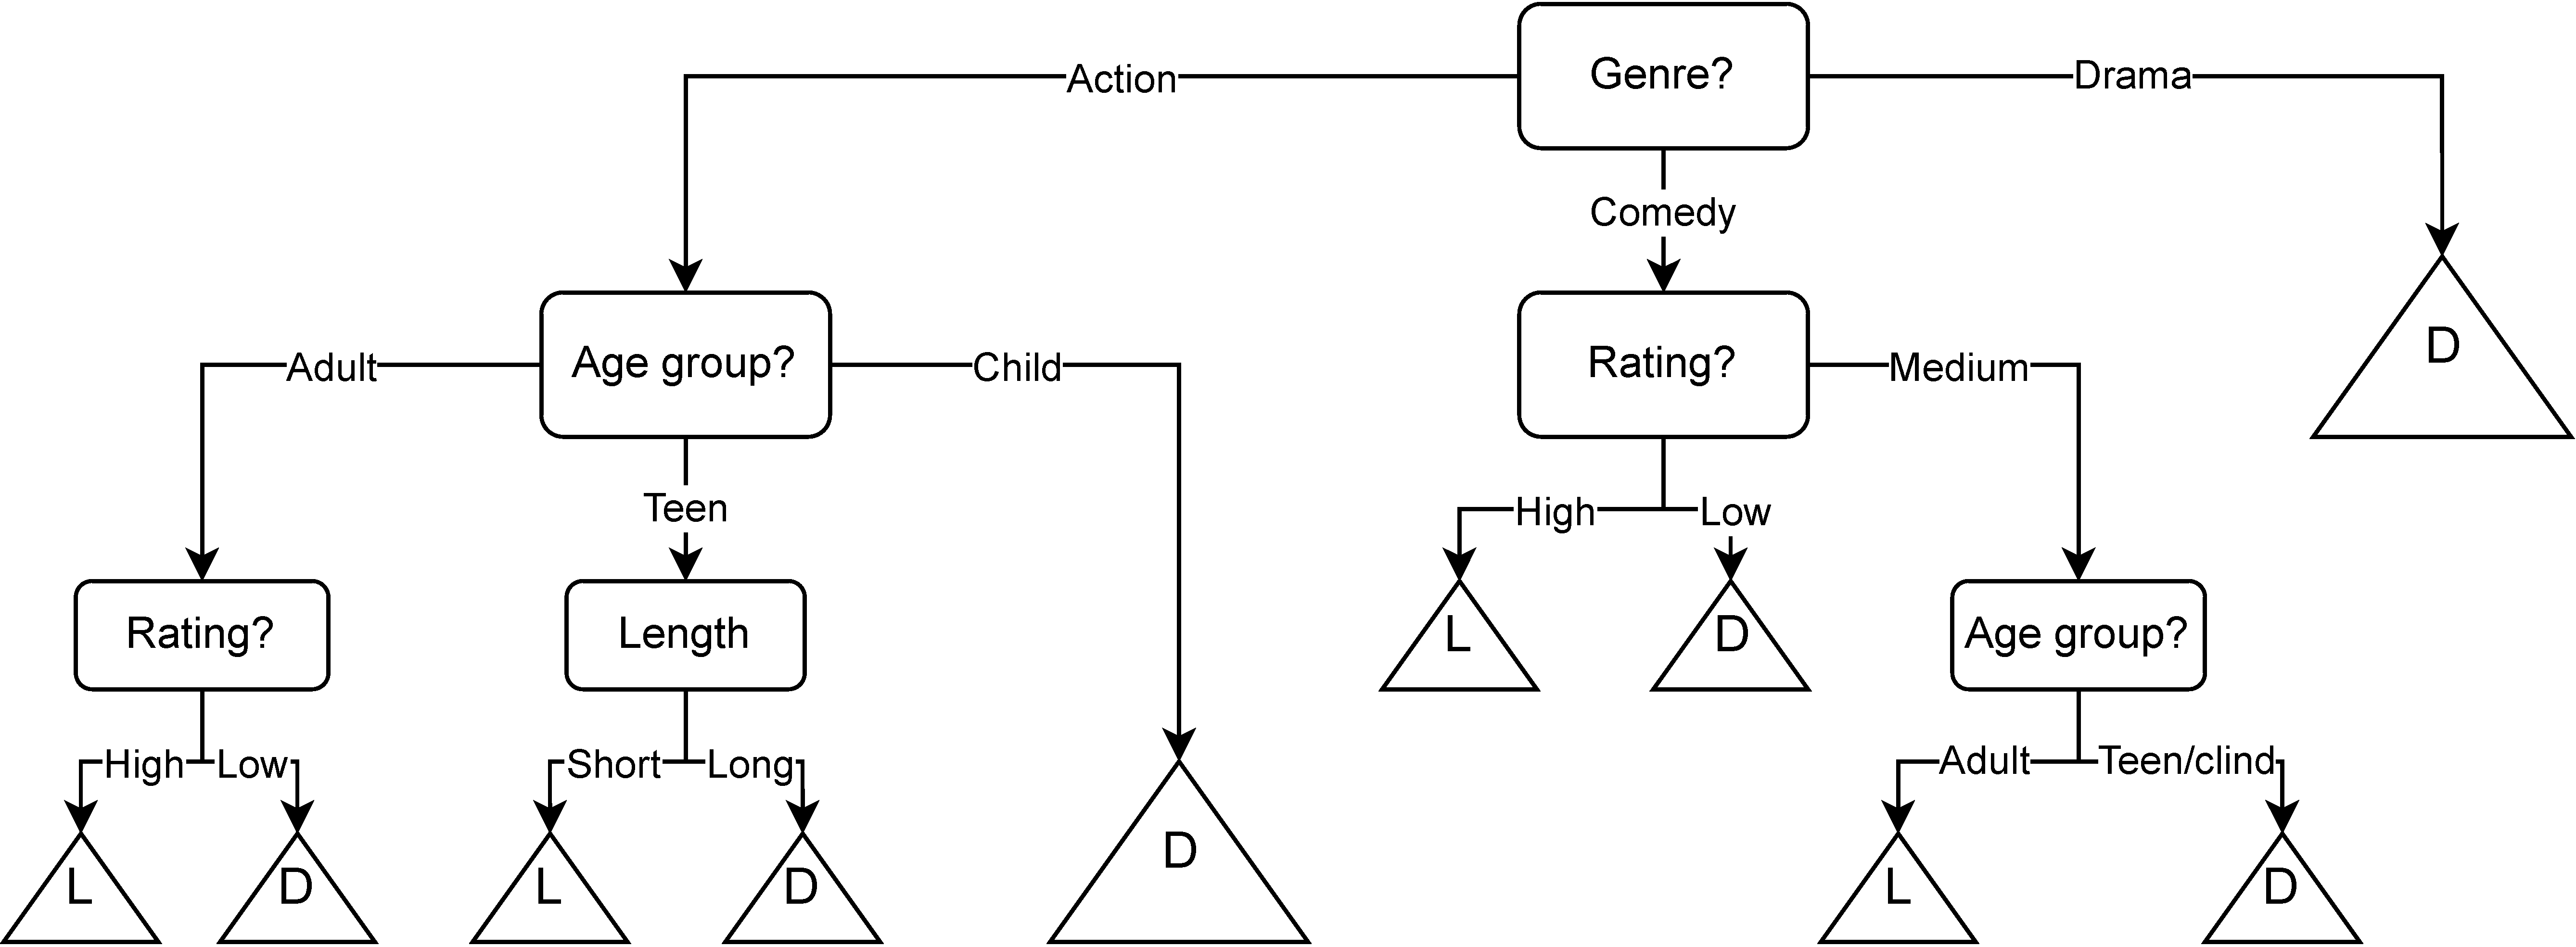
\includegraphics[width=\textwidth]{figures/diagrams/article_decision_tree.pdf}
    \caption{Example of decision-tree}
    \label{fig:decision_tree}
    \end{figure}
\end{center}

\subsection{K-Nearest Neighbor method}
K-Nearest Neighbor (KNN) belongs to vector space methods that are used in N dimensional environments (see section 3 for more details). It is highly used and has better results than decision-tree in the majority of data sets\cite{KNN}.

But before using KNN, we should collect data from user interactions (e.g. user likes) into a user-item matrix. The example of the user-item matrix is shown in Figure 2. In example, user has different amount of 

\begin{table}[h]
    \centering
    \begin{tabular}{|c|c|c|c|c|}
        \hline
        \textbf{Users} & \textbf{Movie 1} & \textbf{Movie 2} & \textbf{Movie 3} & \textbf{Movie 4} \\        
        \hline
        User 1 & 3 & 0 & 1 & 2\\
        \hline
        User 2 & 0 & 5 & 5 & 3\\
        \hline
        User 3 & 5 & 1 & 1 & 2\\
        \hline
        User 4 & 0 & 0 & 5 & 0\\
        \hline
    \end{tabular}
    \caption{User-item matrix}\label{tab:user_item_matrix}
\end{table}

\begin{table}[h]
    \centering
    \begin{tabular}{|c|c|c|c|c|}
        \hline
        \textbf{Genres} & \textbf{Movie 1} & \textbf{Movie 2} & \textbf{Movie 3} & \textbf{Movie 4} \\        
        \hline
        Action  & 1 & 0 & 0 & 1\\
        \hline
        Romance & 0 & 1 & 1 & 0\\
        \hline
        Comedy  & 1 & 1 & 1 & 0\\
        \hline
        Horror  & 0 & 0 & 0 & 1\\
        \hline
    \end{tabular}
    \caption{Genre-movie matrix}\label{tab:genre_movie_matrix}
\end{table}

\newcommand{\cosinesimilarity}{%
    \begin{equation}
    \text{similarity} = \cos(\theta) = \frac{\vec{A} \cdot \vec{B}}{||\vec{A}|| \times ||\vec{B}||} = \frac{\sum_{i=1}^{n} A_i B_i}{\sqrt{\sum_{i=1}^{n} A_i^2} \times \sqrt{\sum_{i=1}^{n} B_i^2}}
    \end{equation}
}
\begin{table}[h]
    \centering
    \begin{tabular}{|c|c|c|c|c|}
        \hline
         & Movie 1 & Movie 2 & Movie 3 & Movie 4 \\        
        \hline
        Movie 1 &1		&0.5	&0.5	&0.5\\
        \hline	
        Movie 2 &0.5	&1      &1		&0	\\
        \hline
        Movie 3 &0.5	&1		&1		&0	\\
        \hline
        Movie 4 &0.5	&0		&0		&1	\\
        \hline
    \end{tabular}
    \caption{Cosine similarity matrix}\label{tab:cosine_similarity_matrix}
\end{table}
\section{Comparative Analysis of Content-Based Filtering Algorithms}\label{sec:dataset_analysis}

\subsection{Dataset description} % TODO
The analysis will be conducted on Book Crossing dataset collected by Cai-Nicolas Ziegler and edited by Arthur Forte \cite{Dataset}. The dataset contains 272,679 interactions from 2,946 users on 17,384 books. The users with less than 10 interactions were deleted from the original dataset by Arthur Forte, therefore there are no users with small amount of iterations.

\subsection{Evaluation Metrics} %TODO
For the metrics F1 Score and Root mean square error (RMSE) is used. Additionally, build time and prediction time is measured. We analyse maximum build and prediction time and prediction time is measured not for one item, but for the collection of items related to one user, therefore the values could be high. Also, the analysis is prepared in a test environment, real applications use some optimization techniques that greatly reduce the time.

F1 Score is calculated using Equation \eqref{equ:f1_score}, additional elements illustrated in Equations \eqref{equ:f1_precision_recall}. The formula consists of 3 main values: number of true positive, false positive and false negative results. Prediction is better if the F1 Score is closer to 1 \cite{F1Score}. The dataset has ratings from 1 to 10, therefore we use F1 weighted Score. For a better analysis, we calculate two F1 scores, one using ratings 1 to 10 and second placing each rating into three groups: “Low” (1-3), “Middle” (4-6) and “High” (7-10). It is nearly impossible to predict rating from 1 to 10, but with group diving the results are much better.
\begin{equation}
        \text{F1 Score} = \frac{2 \cdot \text{precision} \cdot \text{recall}}{\text{precision} + \text{recall}}\label{equ:f1_score}
\end{equation}
\begin{align}
        &\text{precision} = \frac{\text{TP}}{\text{TP} + \text{FP}} &
        \text{recall} = \frac{\text{TP}}{\text{TP} + \text{FN}} &\label{equ:f1_precision_recall}
\end{align}

RMSE formula is illustrated in Equation \eqref{equ:rmse}. We also measure two RMSE values, one with 1 to 10 rating (10 categories) and the other with three groups. Comparing to F1 Score, RMSE prediction is better if RMSE value is closer to zero \ref{RMSE}.
\begin{equation}
    \text{RMSE} = \sqrt{\frac{1}{n} \sum_{i=1}^n (y_i - \hat{y}_i)^2}\label{equ:rmse}
\end{equation}
\subsection{Results} %TODO
The score results are illustrated in Table \ref{tab:analysis_scores}. Analysis was performed using Decision tree (C4.5) algorithm, 

Analysis was performed using the Decision tree (C4.5) algorithm, K-Nearest Neighbor (with different distance calculation algorithms, given in the table) and Random prediction, to compare the quality of recommendations. Although the correlation between F1 score and RMSE was not perfect all the time, the general trend is quite similar. Additionally, there is a correlation between 3 categories and 10 categories diving. RMSE values for 3 categories are about 4.4 times better, while F1 scores are only 2.5 times better. Interesting, that for Random prediction the improvement for both category types is similar (3.5 and 3.6 times respectively). Thanks to these patterns, it can be determined that F1 Score for this dataset better visualizes the actual predictive performance.

Due to the analysis, KNN with Manhattan distance showed the best predictive result for the used dataset. However, the difference between KNN with Manhattan distance, Decision tree and KNN with Hellinger distance is smaller than 1%, therefore all three methods have similar performance. KNN with Euclidean and Levenshtein distances have slightly smaller scores, but the difference with Manhattan distance is less than 4%. Angular (the improvement of cosine similarity) and Chebyshev distances have 10% lower prediction performance, compared to Manhattan distance. Therefore, the use of these distances are not recommended with the used dataset. KNN with Minkowski distance have smaller results compared to random prediction, thus the use of this distance on this dataset is not recommended.

All algorithms besides KNN with Minkowski distance have significantly better results than random prediction. Therefore, they can be used for a recommendation system for this dataset.


\begin{table}[h]
    \centering
    {\small
    \begin{tabular}{|c|c|c|c|c|}
        \hline
         & F1 Score (10) & RMSE (10) & F1 Score (3) & RMSE (3) \\        
        \hline
        Decision tree       & 0.360 & 1.352 & 0.858& 0.300\\
        \hline
        KNN (Euclidean)     & 0.367 & 1.402 & 0.847 & 0.315\\
        \hline
        KNN (Angular)       & 0.251 &1.870 & 0.750 & 0.425\\
        \hline
        KNN (Chebyshev)     & 0.287	& 1.641& 0.790 & 0.367\\
        \hline
        KNN (Hellinger)     & 0.398 & 1.351 & 0.856 & 0.304\\
        \hline
        KNN (Levenshtein)   & 0.332 & 0.363 & 0.827 & 0.363\\
        \hline
        KNN (Manhattan)     & 0.358 & 1.357 & 0.863 & 0.287\\
        \hline
        KNN (Minkowski)     & 0.104	& 3.387 & 0.286 & 0.925\\
        \hline
        Random Recom.       & 0.107 & 4.025 & 0.395 & 1.147\\
        \hline
    \end{tabular}
    }
    \caption{F1 Score and RMSE Results}\label{tab:analysis_scores}
\end{table}

The second necessary aspect of algorithms is time required for building the model (decision tree or matrix) and prediction results (recommendation time). The values of these aspects are illustrated in Table \ref{tab:analysis_performence}. To analyse performance we shouldn't compare actual values (seconds, milliseconds), but the difference of required time to each algorithm. The actual time depends on hardware capabilities and would be different in each application. Therefore we will measure the time in “abstract units”.

Due to the results, maximum build time has a Decision tree (C4.5) algorithm. This is due to the complexity of constructing a tree. All KNN algorithms have the smallest building value. However, we should build the model only once (and only improve it then), so the high build time often isn't a problem.

On the other hand, prediction time is really necessary and affects customer experience. Besides random prediction, the smallest maximum prediction time has a Decision tree (C4.5) algorithm which is about 20 times lower than any other KNN algorithm. Comparing KNN algorithms, Angular, Chebyshev, Euclidean and Manhattan distances have the lowest values, while Hellinger and Minkowski have significantly higher results and Levenshtein distance showed the worst time performance with 123518 abstract units.

Due to the overall analysis, for this dataset it is better to use Decision tree (C4.5) or KNN with Manhattan distance algorithms. The use of KNN is strongly discouraged due to prediction performance, and the use of KNN with Levenshtein, Hellinger and Minkowski distances is also not recommended due to high prediction time.

\begin{table}[h]
    \centering
    {\small
    \begin{tabular}{|c|c|c|c|c|}
        \hline
            & Max Build Time & Max Prediction Time \\        
        \hline
        Decision tree       & 588 & 10\\
        \hline
        KNN (Euclidian)     & 3 & 248\\
        \hline
        KNN (Angular)       & 3 & 170\\
        \hline
        KNN (Chebyshev)     & 3 & 255\\
        \hline
        KNN (Hellinger)     & 3 & 2337\\
        \hline
        KNN (Levenshtein)   & 3 & 123518\\
        \hline
        KNN (Manhattan)     & 3 & 313\\
        \hline
        KNN (Minkowski)     & 3 & 1714\\
        \hline
        Random Recom.       & - & 1\\
        \hline
    \end{tabular}
    }
    \caption{Performence metrics}\label{tab:analysis_performence}
\end{table}
\section{Advantages and disadvantages of content-based filtering}\label{sec:cbf_advantages_disadvantages} %TODO : could be rewrited to usecases of CBF

\subsection{Advantages} %TODO

\subsection{Limitations} %TODO


\section{Conclusion}\label{sec:conclusion}

\bibliography{bibliography/references}
\bibliographystyle{unsrt}
\end{document}
